%%%%%%%%%%%%%%%%%%%%%%%%%%%%%%%%%%%%%%%%%%%%%%%%%%%%%%%%%%%%
% SCRUM-14 DATABASE AND DIGITAL STORAGE ARCHITECTURE
% Responsible member: Nhu Quan
%%%%%%%%%%%%%%%%%%%%%%%%%%%%%%%%%%%%%%%%%%%%%%%%%%%%%%%%%%%%

\subsection{Database and Digital Storage Architecture}

This section defines the proposed database and digital storage architecture
for the AI-powered Film Photography Platform.

\subsubsection{Database Architecture}

PostgreSQL is proposed as the primary relational database for storing
structured system data. The database stores information related to users,
films, Film Labs, services, orders, reviews, community activities, and
film scan metadata.

The Backend API acts as the main access layer between the mobile/web
applications and PostgreSQL. Client applications send API requests to the
Backend API, which handles business logic, authentication, authorization,
and database access.

The main data entities include:

\begin{itemize}
    \item User
    \item Film
    \item Film Lab
    \item Service
    \item Order
    \item Review
    \item Community
    \item Film Scan Metadata
\end{itemize}

\subsubsection{Digital Storage Architecture}

Digital film scans are separated from structured relational data.
PostgreSQL stores scan metadata such as file name, file type, file size,
file path, and related information, while the actual film scan files are
stored in cloud storage.

The proposed architecture uses the Backend API as the access layer for
uploading and retrieving film scans. This approach separates structured
data management from large media file storage and supports scalability
and secure file access.

\subsubsection{Data Access and Security}

The Backend API controls access to both PostgreSQL and cloud storage.
Authentication and authorization mechanisms are applied before users can
access protected data or digital film scans.

This architecture provides centralized data access, supports backup and
recovery, and allows the storage system to scale as the number of users
and film scans increases.

\begin{figure}[htbp]
    \centering
    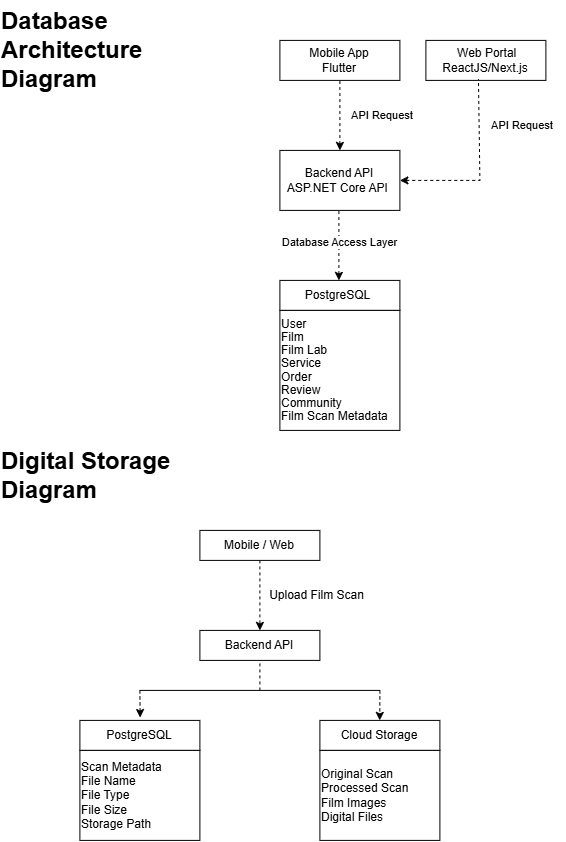
\includegraphics[width=0.85\textwidth]{sections/14-database-storage-architecture.png}
    \caption{Database and Digital Storage Architecture}
    \label{fig:database-storage-architecture}
\end{figure}
